\section{Breitensuche}
\label{subsec:module.Suchalgorithmen.Breitensuche}

\begin{figure}[H]
\centering
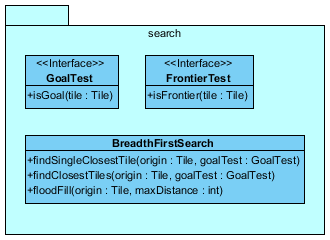
\includegraphics[width=0.7\textwidth]{91_bilder/BFS}
\caption{Breitensuche Klassendiagramm}
\label{fig:BFS}
\end{figure}

\begin{figure}[H]
\centering
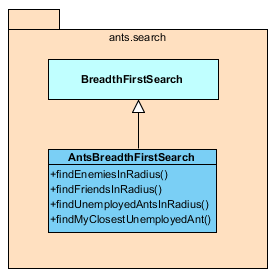
\includegraphics[width=0.5\textwidth]{91_bilder/BFSants}
\caption{Breitensuche Ants-spezifisch}
\label{fig:BFSants}
\end{figure}
Die Breitensuche (engl. breadth-first search (BFS)) war eine der Neuimplementierungen w�hrend der Bachelorarbeit. Man k�nnte die BFS auch f�r die Pfadsuche verwenden, dies w�re aber sehr ineffizient. Wir verwenden diese Suche vielmehr f�r die Umgebung einer Ameise oder eines H�gels zu analysieren. Sie wurde generisch implementierte, so dass sie vielseitig einsetzbar ist. So k�nnen zum Beispiel mittels 'GoalTest' je nach Anwendungsfall die Tiles beschrieben werden welche gesucht sind. Folgende Breitensuche findet die Ameise welche am n�chsten bei einem Food-Tile <r:20,c:16> ist. Sie wird initialisiert indem im Konstruktor die Spielkarte mitgegeben wird, welche durchforscht wird. Zus�tzlich gilt die Einschr�nkung das die Breitensuche nur 40 Tiles durchsuchen darf, was einem Radius von zirka 7 entspricht. Falls keien Ameise gefunden wird gibt der Algorithmus NULL zur�ck.

\begin{verbatim}
AntsBreadthFirstSearch bfs = new AntsBreadthFirstSearch(Ants.getWorld());
Tile food = new Tile(20,16);
Tile antClosestToFood = bfs.findSingleClosestTile(food, 40, new GoalTest() {
      @Override
      public boolean isGoal(Tile tile) {
          return isAntOnTile(tile);
      }
  });
\end{verbatim}

Es ist auch m�glich mehrere Tiles zur�ck zu bekommen. Dazu wird die Methode findClosestTiles(...) aufgerufen.
\newline
\newline

Der gleiche Alogrithmus kann aber auch alle passierbaren Tiles in einem gewissen Umkreis zur�ckgeben. Dies haben wir unteranderem beim Initialisieren der DefendHillMission verwendet. Wir berechnen beim Erstellen der Mission die passierbaren Tiles rundum den H�gel. Runde f�r Runde pr�fen wir diese Tiles auf gegnerische Ameisen um die entsprechenden Verteidigungsmassnahmen zu ergreifen. Der Parameter controlAreaRadius2 definiert den Radius des 'Radars' und kann je nach Profile unterschiedlich eingestellt werden.

\begin{verbatim}
public DefendHillMission(Tile myhill) {
    this.hill = myhill;
    BreadthFirstSearch bfs = new BreadthFirstSearch(Ants.getWorld());
    tilesAroundHill = bfs.floodFill(myhill, controlAreaRadius2);
}
\end{verbatim}